\documentclass[12pt]{article}
\usepackage[letterpaper, margin=0.75in]{geometry}
\usepackage{tabularx}
\usepackage{graphicx}
\usepackage{titling}
\usepackage[makeroom]{cancel}
\usepackage{color}

\pretitle{\begin{center}\LARGE
\includegraphics[width=10cm]{../images/logo.png}\\[\bigskipamount]}
\posttitle{\end{center}}

\begin{document}

\begin{center}

\includegraphics[width=10cm]{../images/logo.png}
\end{center}

\begin{center}
\noindent{\LARGE Conceptual Physics \\ Lecture Notes}\footnote{DISCLAIMER: These notes contain typos.}

\vspace{0.1in}
\noindent{Katherine Quinn}
\end{center}

\noindent These lecture notes relate to part one of this course. It is material covered in classes 1 through 6:
\begin{enumerate}
\item Philosophy of Science
\item Units and Scientific Notation
\item Kinematics
\item Graphs
\item Forces
\item Energy and Momentum
\end{enumerate}

\noindent Each part of these notes lists the relevant readings, and then summarizes the relevant material with sample problems.\footnote{DISCLAIMER: The worked examples may also contain typos. I apologize for the vast quantity of typos, but I haven't had time to thoroughly read through the notes and correct every one of them.} Note that while the same material is covered in class 7, the review class, there will be no lecture as that class will be purely reserved for co-op problems and questions.

\section{Philosophy of Science}

\begin{itemize}
\item \textbf{Ideology:} Set of of ideas.
\item \textbf{Scientific theories:} Set of \textit{falsifiable} ideas. Explanation for patterns that has predictive value and survived a broad set of empirical tests.
\item \textbf{Science:} Method used to explain and make predictions by subjecting theories to skepticism and rigorous testing. It is the cycle between \textit{theory} and \textit{experiment}
\item \textbf{Experiment:} Need to be reproducible for anyone with the same skills and equipment. Should get the same result for the same experiment.
\item \textbf{Hypothesis:} Statement of interest that can be empirically tested. Becomes a ``theory" when it has been verified by multiple sources in various ways.
\item \textbf{Model:} Representation of something. Models can be simple (Newtonian model of solar system) or complicated (quantum mechanical view of the atom)
\end{itemize}

When an experiment or observation is made that cannot be explained by current models and theories, then the models and theories need to change.

Science is done by people. This presents many challenges, as institutions of science are as prone to bias, misrepresentations, misuse, and corruption as any other man-made institution:
\begin{itemize}
\item People have a tendency to double down on their opinions, rather than change them, when faced with contradicting evidence
\item People have biases and perspectives that prevent objectivity
\item People want the glory of a new discovery, therefore little effort is put into verifying experimental results.
\item ``Science" is seen as pure and objective, and associated with hard reasoning. It is therefore difficult to challenge an ``expert scientist" who can wield their titled when questioned (about motives, intention), conferring a position of authority
\item Science funding often dictates science project.
\end{itemize}

The founding principles behind science are that nature is understandable, and if we apply the cycle of theory and experiment we will be able to understand everything. Is this in and of itself an ideology?

\section{Units and Scientific Notation}

\noindent \textbf{Readings:}
\begin{enumerate}
\item Chapter 0 (Sections 5, 8 and 9) of \textit{Light and Matter}
\end{enumerate}
	
\noindent \textbf{\large Units}
	
\noindent \textbf{Dimensional Analysis:} For physical quantities to be added or compared, they must be expressed in identical \textit{units}

\noindent \textbf{Metric System:} Base 10 system of measurement.

\begin{enumerate}
	\item \textbf{Time:} second (s)
	\item \textbf{Distance:} meter (m)
	\item \textbf{Mass:} gram (g)
\end{enumerate}

Note: A pound is actually a unit of \textit{force}, not mass: If you were on the moon, your weight in pounds would be less but your mass would be the same.
\vspace{0.1in}

\noindent \begin{tabularx}{\textwidth}{X | X}
	Fundamental Units & Compound Units \\ \hline
	Quantities that cannot be broken down (time, distance, mass) & Quantities composed of fundamental quantities
\end{tabularx}

\vspace{0.1in}
\noindent \textbf{Metric Prefixes:} Since the system is base 10, there are prefixes associated with multiples of 10. The most common ones are:
\vspace{0.1in}

\noindent \begin{tabularx}{\textwidth}{ X X X X X X }
	kilo & (none) & centi & mili & micro & nano \\
	k & (none) & c & m & $\mu$ & n \\
	$\times$ 1000 & (none) & $/$ 100 & $/$ 1000 & $/$ million & $/$ billion \\
	$10^3$ & $10^0$ & $10^{-2}$ & $10^{-3}$ & $10^{-6}$ & $10^{-9}$ \\
	1000 & 1 & 0.01 & 0.001 & 0.000001 & 0.000000001 
\end{tabularx}
\clearpage
\noindent \textbf{\large Converting Units}

We convert units using \textit{conversion factors.}

\noindent\textbf{Example} Convert 50 miles to km. Use the following conversion:
\begin{eqnarray}
1~mile = 1.5~km
\end{eqnarray}

If we divide both sides of the equation by miles, then we get:
\begin{eqnarray}
\frac{1~mile}{1~mile} = \frac{1.5~km}{1~mile} = 1
\end{eqnarray}

If we divide by kilometers instead, we get:
\begin{eqnarray}
\frac{1~mile}{1.5~km} = \frac{1.5~km}{1.5~km} = 1
\end{eqnarray}

knowing this, we can construct the equation:
\begin{eqnarray}
50~\cancel{miles}\times\frac{1.5~km}{1~\cancel{mile}} = 75~km
\end{eqnarray}

\noindent\textbf{Example} Convert 10 feet to inches. Use the conversion factor:
\begin{equation}
1~ft = 12~inches
\end{equation}

And so we can write out:
\begin{eqnarray}
10~\cancel{ft}\times\frac{12~inches}{1~\cancel{ft}} = 120~inches
\end{eqnarray}


\noindent\textbf{Example} Convert 18~km/h to m/s, using the following conversion factors:
\begin{eqnarray}
1~km &=& 1000~m \\
1~h &=& 60~min \\
1~min &=& 60~s
\end{eqnarray}

We get a large formula:
\begin{eqnarray}
\frac{18~\cancel{km}}{1~\cancel{h}}\times\frac{1000~m}{1~\cancel{km}}\times\frac{1~\cancel{h}}{60~\cancel{minutes}}\times\frac{1~\cancel{min}}{60~s} = \frac{18000~m}{3600~s} = \frac{180~m}{36~s} = \frac{30~m}{6~s} = 5~m/s
\end{eqnarray}

\noindent\textbf{\large Scientific Notation}

\textbf{Scientific Notation:} expressing numbers as a product of:

\begin{center}
A number between 1 and 10 \textit{and} 10 to a power
\end{center}

For big numbers, the exponent is \textit{positive}
\begin{eqnarray}
31.4 &=& 3.14 \times 10 = 3.14\times 10^1 \\
314 &=& 3.14 \times 100 = 3.14 \times 10^2 \\
3140 &=& 3.14 \times 1000 = 3.14 \times 10^3
\end{eqnarray}

For small numbers, the exponent is \textit{negative}. 
\begin{eqnarray}
0.314 &=& 3.14 \div 10 = \frac{3.14}{10} = 3.14 \times 10^{-1}\\
0.0314 &=& 3.14 \div 100 = \frac{3.14}{100} = 3.14\times 10^{-2} \\
0.00314 &=& 3.14 \div 1000 = \frac{3.14}{1000} = 3.14 \times 10^{-3}
\end{eqnarray}

If the number is about 1, the exponent is \textit{zero}.
\begin{eqnarray}
3.14 = 3.14 \times 1 = 3.14\times 10^0
\end{eqnarray}

A number can be switch from the numerator to the denominator, or the denominator to the numerator, and in doing so the exponent changes sign:
\begin{eqnarray}
\frac{4}{10^{5}} &=& \frac{4\times 10^{-5}}{1} \\
\frac{2\times 10^{-4}}{1} &=& \frac{2}{10^4}
\end{eqnarray}

When multiplying two numbers, the powers \textit{add}:
\begin{eqnarray}
10^{2}\times 10^{3} &=& 10^{2+3} = 10^5 \\
10^{6} \times 10^{-1} &=& 10^{6-1} = 10^5
\end{eqnarray}

\section{Kinematics}
	
\noindent \textbf{Readings:}
\begin{enumerate}
\item Chapter 2 (Sections 1, 2 and 5) of \textit{Light and Matter}
\item Chapter 2 (Sections 1 to 5) of \textit{College Physics}
\item Chapter 3 (Sections 1 to 4, 6) of \textit{Light and Matter}
\end{enumerate}
	
\noindent \textbf{\large Describing Motion}

\noindent \textbf{Kinematics:} Study of motion without considering cause.
\vspace{0.1in}

\noindent \begin{tabularx}{\textwidth}{X | X}
 \textbf{No Direction} & \textbf{Direction} \\
 \hline
 \textbf{Distance} \newline \textit{Length of path traveled.} &  \textbf{Displacement} \newline \textit{Distance between final and initial position.} \begin{equation}
 \Delta x
 \end{equation}
 \\ 
 \textbf{Speed} \newline \textit{Distance traveled divided by time to travel} \begin{equation}
 speed = \frac{distance}{time}
 \end{equation} & \textbf{Velocity} \newline \textit{Displacement divided by time}. \begin{equation}
 velocity = \frac{displacement}{time} = \frac{\Delta x}{\Delta t}
 \end{equation}
\end{tabularx}
\vspace{0.1in}

\noindent \textbf{Example:} A car travels 15 miles in 10 minutes. What is its speed?
\begin{eqnarray}
speed = \frac{distance}{time} = \frac{15~miles}{10~min} = 1.5~miles/min\left(=\frac{1.5~miles}{\cancel{min}}\times\frac{60~\cancel{min}}{1~hour}=90~miles/h\right)
\end{eqnarray}

\noindent \textbf{Example:} A car is traveling at 75 miles/hour. How long does it take to travel a distance of 150 miles?
\begin{eqnarray}
150~miles \times \frac{1~h}{75~miles} = \frac{150~hours}{75} = 2~hours
\end{eqnarray}

\noindent \textbf{Example:} You walk 10~m down a hallway, then turn around and walk back to where you started in 20~s.

Distance: 20~m

Displacement: 0~m

Speed: 1~m/s

Velocity: 0~m/s

\noindent \textbf{Acceleration:} The rate at which \textit{velocity} changes.
\begin{eqnarray}
acceleration = \frac{change~in~velocity}{change~in~time} = \frac{\Delta v}{\Delta t}
\end{eqnarray}

\noindent\textbf{Example:} A loaded freight train, traveling at 60~miles/hour, comes to a full stop over the course of an hour. 
\begin{eqnarray}
acceleration = \frac{\Delta v}{\Delta t} = \frac{-60~miles/hour}{1~hour} = -60~miles/h^2
\end{eqnarray}

\noindent \textbf{Example:} A car accelerates from rest to 60~miles/hour in 2 seconds. What is its acceleration?
\begin{eqnarray}
a = \frac{\Delta v}{\Delta t} &=& \frac{60~miles/h}{2~\cancel{s}}\times\frac{3600~\cancel{s}}{1~h} = 108,000~miles/h^2 \\
&=& \frac{60~miles/\cancel{h}}{2~s} \times \frac{1~\cancel{h}}{3600~s} = 0.008 ~miles/s^2
\end{eqnarray}

\noindent \textbf{\large Positive and Negative Signs}

Displacement, velocity and acceleration have a \textit{direction}, and so will sometimes have a positive or negative sign.

\begin{itemize}
	\item \textbf{Positive:} In the \textit{same} direction of the reference frame.
	\item \textbf{Negative:} In the \textit{opposite} direction of the reference frame.
\end{itemize}

\noindent \textbf{Example:} a train track where location $x=0$ is given by a station, where West is a negative direction and East is a positive direction. Then a train 14~miles west of the station would be located at $x = -14~miles$.

\begin{center}\input{../images/train_position.pdf_tex}\end{center}

\noindent \textbf{\large Equations}

Note: When considering multiple points (positions, velocities, points in time) \textit{subscripts} are used.

For multiple points:
\begin{equation}
t_0, t_1, t_2, etc.
\end{equation}

For only 2 points:
\begin{equation}
t_i, t_f ~\quad \texttt{or} \quad t_0, t_f
\end{equation}

Change in something:
\begin{eqnarray}
\underbrace{\Delta t}_{change} = \underbrace{t_f}_{final} - \underbrace{t_i}_{initial}
\end{eqnarray}

For motion with constant acceleration, there are simple equations we can use.

\begin{itemize}
	\item Relate \textit{acceleration}, \textit{velocity} and \textit{time}.
	\begin{eqnarray}
	a = \frac{\Delta v}{\Delta t} \Rightarrow & &\Delta v = a\times \Delta t\\
	& & v_f - v_i = a\times t \\
	& & v_f = v_i + a\times t
	\end{eqnarray}
	\item Relate \textit{position}, \textit{velocity}, \textit{acceleration} and \textit{time}
	\begin{eqnarray}
	v = \frac{\Delta x}{\Delta t} \Rightarrow & & \Delta x = v \times \Delta t \\
	& & x_f - x_i = v\times t \\
	& & x_f = x_i + v\times t +\underbrace{\frac{1}{2}at^2}_{graphs}
	\end{eqnarray}
	\item For those who are good at algebra:
	\begin{eqnarray}
	v_f^2 = v_i^2 + 2a(x_f-x_i)
	\end{eqnarray}
\end{itemize}

\noindent A useful way of relating the kinematic equations is through:
\begin{center}
\input{../images/constantA.pdf_tex}
\end{center}

\noindent \textbf{Example:} You see rock fall from the top of a $20~m$ building. Acceleration due to gravity is $9.81~m/s^2$ down ($-10~m/s^2$). How long does it take to fall?
\begin{eqnarray}
x_f &=& x_i + v_i\times t + \frac{1}{2}a\times t^2 \\ 
0~m &=& 20~m + \frac{1}{2}(-10~m/s^2)\times t^2 \\
0~m &=& 20~m - 5~m/s^2\times t^2 \\
-20~m &=& -5~m/s^2\times t^2 \\
\frac{-20~m}{-5~m/s^2} &=& t^2 \\
t &=& \sqrt{4}s = 2~s
\end{eqnarray}

\section{Graphs}
	
\noindent \textbf{Readings:}
\begin{enumerate}
\item Chapter 2 (Section 3) of \textit{Light and Matter}
\item Chapter 2 (Section 8) of \textit{College Physics}
\end{enumerate}
	
\noindent \textbf{\large Average vs. Instantaneous:}
\begin{itemize}
	\item \textit{Average Velocity/Speed:}  Velocity/Speed averaged over a period of time.
	\item \textit{Instantaneous Velocity/Speed:} Velocity/Speed at an instant in time.
\end{itemize}

\textbf{Example:} You travel 100 miles in 2 hours. Sometimes on the highway going 70 miles/hour, sometimes stopped in traffic.
\begin{itemize}
	\item Average speed: $100~miles/2~hours$ = 50 miles/hour.
	\item Instantaneous speed: 70 miles/hour on the highway, 0 when stopped.
\end{itemize}
	
\noindent \textbf{\large Graph:} A way of visually representing a relation between variables (quantities).

A graph has 2 axes: Horizontal (``independent" variable) and Vertical (``dependent" variable). When labelling a graph, we say is it ``Vertical variable" versus ``Horizontal variable".

In this course, time will always be on the horizontal axis, with position/velocity/acceleration on the vertical.

\textbf{Slope:} Describes how the dependent variable changes when the independent one does. It is described through a ratio.
\begin{center}\input{../images/graph.pdf_tex}\end{center}

The sign of the slope is important: positive = up and to the right, negative = down and to the right.

The \textit{area} under a graph is found by looking at the space between the curve and the horizontal axis. Just like slope, area can be positive or negative.

\begin{center}\input{../images/positive_negative_area.pdf_tex}\end{center}

For kinematics, time is independent; it is therefore represented by the horizontal axis. This convention is very useful for relating kinematic quantities: Position, displacement, velocity \& speed, and acceleration can all be related to one another through graphs.

\noindent\textbf{\large Position versus Time}

The slope of a position versus time graph is given by:
\begin{eqnarray}
slope = \frac{\Delta Dependent}{\Delta Independent} = \frac{\Delta x}{\Delta t} = velocity \nonumber
\end{eqnarray}

For example, the graph below shows an object starting at position $x=2~m$ and slowly increasing its position in time at a rate of 1~m/s. Its velocity is thus 1~m/s, which is the slope of the graph.

\begin{center}\input{../images/post_vs_time.pdf_tex}\end{center}

Since slope is a \textit{ratio}, it doesn't matter how we calculated it:
\begin{eqnarray}
slope = \frac{\Delta x}{\Delta t} &=& \frac{8-3~m}{6-1~s} = \frac{5}{5} m/s = 1~m/s\nonumber\\
&=& \frac{7-5~m}{5-3~s} = \frac{2}{2} m/s = 1~m/s\nonumber
\end{eqnarray}

Position vs. Time graphs that are straight lines are special, in that the \textit{instantaneous} and \textit{average} velocities are the same. However, when dealing with \textit{curved} graphs, the two can be different. The slope of the \textit{tangent} line indicates the \textit{instantaneous} velocity.

\begin{center}\input{../images/post_vs_time_tangent.pdf_tex}\end{center}


\textbf{Checking Units:} The slope of a position vs. time graph is given by $\frac{\Delta x}{\Delta t}$, which has units of distance/time - the same as velocity.
\vspace{0.2in}

\noindent\textbf{\large Velocity versus Time}

The slope of a velocity vs. time graph is given by:
\begin{eqnarray}
slope = \frac{\Delta Dependent}{\Delta Independent} = \frac{\Delta v}{\Delta t} = acceleration \nonumber
\end{eqnarray}

\textbf{Checking Units:} The slope is given by a change in velocity per change in time, which has units of (distance/time)/time = distance/time/time = distance/time$^2$ = acceleration.

Just as with position vs. time, the \textit{tangent} to a point on a velocity vs. time graph has meaning: It is the \textit{instantaneous} acceleration.

Unlike position vs. time, the area under a velocity graph also has physical meaning. If we check units:
\begin{eqnarray}
area = \Delta Dependant \times \Delta Independent = \Delta v &\times & \Delta t \nonumber \\
\textrm{units of: } \frac{distance}{time} &\times & time = distance
\end{eqnarray}

\textbf{Area} of a \textbf{Velocity} vs. Time graph = \textbf{Displacement}

\textbf{Area} of a \textbf{Speed} vs Time graph = \textbf{Distance Traveled}
\vspace{0.2in}

\noindent\textbf{\large Acceleration versus Time}

The slope of an acceleration versus time graph has physical meaning (represents how much the acceleration is changing and is called a jerk, also known as jolt, surge, or lurch) but we won't keep looking at slopes. What we care about is the \textit{area}; since it represents the change in velocity.
\begin{eqnarray}
area = \Delta a &\times & \Delta t \nonumber \\
\frac{distance}{time^2} &\times & time = \frac{distance}{time} = velocity
\end{eqnarray}

To go between position vs. time, velocity vs. time, and acceleration vs. time we look at the slopes and areas of the different graphs. The arrows represent how to go from one to another:

\begin{center}\input{../images/graph_relations.pdf_tex}\end{center}


\section{Forces}

\noindent \textbf{Readings:}
\begin{enumerate}
\item Handout on \textit{The Fundamental Interactions} in the course reader
\item \textit{Light and Matter}, Chapter 4 (all Sections)
\end{enumerate}

\noindent\textbf{4 Known Forces of Nature}

Force: Interaction between objects or particles that causes a push or a pull.
Units of force are
\begin{eqnarray}
N (Newtons) = kg m/s^2 \nonumber
\end{eqnarray}

There are 4 known forces of nature.
\begin{enumerate}
	\item \textbf{Gravity}
		\begin{itemize}
			\item acts on anything with mass/energy. (so everything we know of)
			\item always attractive
			\item has infinite range
			\item stronger when objects are close together, weaker when they are far appart.
			\item stronger when objects are massive, weaker when they have little mass
			\item can be described by Newton's law of gravitation
				\begin{eqnarray}
				F = G \frac{m_1 m_2}{r^2} \nonumber
				\end{eqnarray}
				Where F = force, $G$ is a gravitational constant for the universe, $m_1$ and $m_2$ are the masses attracting each other, and $r$ is the distance separating them.
		\end{itemize}
	\item \textbf{Electromagnetism}
		\begin{itemize}
			\item acts on objects with \textit{electric charge}
			\item has infinite range
			\item attractive and repulsive (like charges repel, opposite charges attract)
			\item Stronger when objects are more charged
			\item stronger when objects are closer together
			\item The electric force can be described by Coulomb's Law
			\begin{eqnarray}
			F = k \frac{q_1 q_2}{r^2} \nonumber
			\end{eqnarray}
			Where F = force, $k$ is a universal constant, $q_1$ and $q_2$ are charges on the two objects that are attracting/repelling each other, and $r$ is the distance separating the two.
			\item The electric force is responsible for many other kinds of forces. Electric forces bind atoms together, and to each other. We are all made up of atoms, and so almost all contact forces (friction, etc.) are the result of the electric force.
		\end{itemize}
	The nuclear forces (strong and weak) act on atomic nuclei:
	\noindent \begin{center}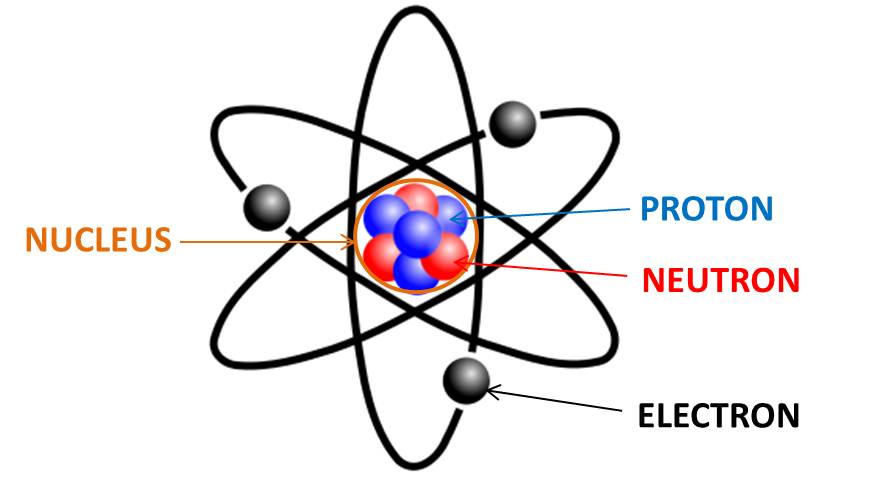
\includegraphics[width=4in]{../images/atom.jpg}\end{center}
	\item \textbf{Strong Nuclear Force}
		\begin{itemize}
			\item Binds atomic nuclei together
			\item Atomic nuclei are positively charged, and so there needs to be come force that prevents the electric force from ripping them apart.
			\item Nuclear force has a finite range, and so this limits the possible size of atomic nuclei.
			\item Acts on all particles with ``colour charge" (there are 3 ``colours")
		\end{itemize}
		
	\item \textbf{Weak Nuclear Force}
	\begin{itemize}
		\item responsible for nuclear decay
		\item acts on very small length scales (a fraction of the size of a proton)
	\end{itemize}
\end{enumerate}

How can particles far away from each other ``communicate" to push/pull away?
\begin{itemize}
	\item Electromagnetism, and nuclear forces (strong and weak) have carrier particles that mediate interactions. Carrier particles are exchanged between other particles.
\begin{center}

\includegraphics{../images/carrier.png}
\end{center}
	\item The size of the carrier particle dictates the range of the interaction.
	\item Electromagnetism: photon (light particle)
	\item Weak nuclear force: W and Z boson
	\item Strong nuclear force: gluon
	\item gravity is different from the rest of the forces, in that the carrier particle (graviton) is theorized but not discovered.
\end{itemize}

Grand unifying theory of physics aims to unite all forces, including gravity. However, this model begins to break down, since the universe is expanding at an increasing rate. This cannot be explained by any of the 4 known forces, and remains an open mystery. ``Dark energy" is a something physicists use a s a place holder for this gap in knowledge.

\textbf{Newton's First Law}

Objects in motion remain in motion, and objects at rest remain at rest, unless they experience an external force. 

Forces cause a change in an object's motion, by causing an acceleration.

\textbf{Newton's Second Law}

The net force on an object is equal to the object's mass times acceleration.
\begin{eqnarray}
	F_{net} = m a \nonumber
\end{eqnarray}

\textbf{Example:} A 2,000~kg car moves forward, with a force of 4,000~N. What is its acceleration?
\begin{eqnarray}
F &=& m a \nonumber \\
4,000~N &=& 2,000~kg \times a \nonumber  \\
\Rightarrow a &=& 2~m/s^2 \nonumber
\end{eqnarray}

Forces are vectors, and can be added together. The net force ($F_{NET}$) on an object is given by the sum of all forces acting on it.

\textbf{Example:} A skydiver weighing 700~N falls to the ground. Friction from the air counteracts her fall, with a force of 300~N. What is her net force?
\begin{eqnarray}
	700~N - 300~N = 400~N~(up) \nonumber
\end{eqnarray}


\textbf{Newton's Third Law}

For every action, there is an equal and opposite reaction.

Objects cannot self accelerate, and so for every closed system, all forces must cancel out. Therefore, there must be an equal and opposite force for everything within a system.

\section{Energy and Momentum}

\noindent \textbf{Readings:}
\begin{enumerate}
\item Handout on \textit{Conservation of Mass and Energy} in the course reader. (All sections except 3)
\item \textit{Light and Matter}, Chapter 13 (Section 1)
\item \textit{College Physics}, Chapter 7 (Sections 1 to 6)
\end{enumerate}

\noindent\textbf{\large Conservation Laws}

Noether's Theorem: For every symmetry of nature, there is a conserved quantity (in an isolated system).

Symmetry: Something which, when changed, leaves the physical laws unchanged (doesn't change the way the universe works).

Examples:
\begin{itemize}
	\item \textbf{Translational symmetry:} Everything would behave the same if the universe was shifted by 10 ft to the left $\rightarrow$ Inertial and conservation of linear momentum
	\item \textbf{Rotational symmetry:} Everything would behave the same if the universe was rotated by $90^0$ $\rightarrow$ Conservation of rotational momentum (things want to stay spinning)
	\item \textbf{Temporal symmetry:} Physics doesn't change with time $\rightarrow$ energy conservation
\end{itemize}

\noindent\textbf{\large Energy}

There are different forms of energy.
\begin{enumerate}
	\item \textbf{Kinetic Energy:} Energy of motion, and the collective energy of the motion of countless small particles (heat).
	\item \textbf{Potential Energy:} ``Stored" Energy
	\begin{itemize}
		\item Chemical potential energy (fuel, food, batteries)
		\item Nuclear potential energy
		\item Gravitational potential energy (from lifting objects in a gravitational field)
		\item Electrical potential energy (capacitors)
		\item Elastic potential energy (stretching springs, rubber bands, etc.)
	\end{itemize}
\end{enumerate}

\textbf{Kinetic Energy}

Energy of motion. The faster something is moving, the greater its kinetic energy. The larger something is, the greater its kinetic energy (when moving at the same speed).

Units of Joules, or $N\times m = kg m^2/s^2)$
\begin{eqnarray}
E_K = \frac{1}{2}mv^2 \nonumber
\end{eqnarray}

There $E_K$ is the kinetic energy, $m$ is the mass of an object, and $v$ is its speed (or magnitude of velocity).

\noindent \textbf{Example:} A 2,000~kg car is moving at 2~m/s. What is its kinetic energy?

\begin{eqnarray}
\frac{1}{2}mv^2 = \frac{1}{2}2000~kg\times\left(2~m/s\right)^2 = 1000\times 4~kg~m/s^2 = 4,000 J
\end{eqnarray}

Heat: Kinetic energy of a collection of moving atoms/molecules. Adding heat to a system makes the particles move faster, removing heat makes particles move slower. Lots of particles, explained with statistics, and a field of physics called statistical mechanics (and thermodynamics).

\textbf{Potential Energy}
``Stored" energy from pushing or pulling objects against a conservative force.

\begin{table}[h!]
     \begin{center}
     \begin{tabularx}{\textwidth}{ |X | X }
      \textbf{Attractive Force} & \textbf{Repulsive Force}
      \\
      -Pulling objects apart increases their potential energy. & -Pushing objects together increases their potential energy. \\
      -Letting them come together decreases their potential energy. & -Letting them fly apart decreases their potential energy.
      \end{tabularx}
      \end{center}
\end{table}

\textbf{Gravitational Potential Energy}

\begin{itemize}
	\item Further apart 2 objects are, the greater their gravitational potential energy.
	\item The more massive 2 objects are, the greater the gravitational force between them and therefore the greater the potential energy from pulling them apart. In a constant gravitational field (like on the surface of the Earth), we have:
\end{itemize}
\begin{eqnarray}
	E_p = g m h \nonumber
\end{eqnarray}

Here $E_p$ is the potential energy, $g$ is the acceleration due to gravity (about $10~m/s^2$ on Earth) and $h$ is the height an object was lifted.

\noindent A 3~kg rock has 60~J of energy. How high above the ground is it?
\begin{eqnarray}
E &=& mgh \\
60~J &=& 3~kg \times 10~m/s^2 \times h \\
60~J &=& 30~kg~m/s^2~h \\
\frac{60~J}{30~kg~m/s^2} &=& h \Rightarrow h = 2~m
\end{eqnarray}

\textbf{Work}

Work is the transfer of energy (except through thermal conduction such as putting a hot and hold object in contact). 2 conditions are required to do work:
\begin{enumerate}
	\item A force.
	\item Travelling a distance parallel to this force.
\end{enumerate}

The greater the force, the more work is done on an object. The longer the distance, the more work is done on an object.
\begin{eqnarray}
	W = F d \nonumber
\end{eqnarray}
Where $W$ is the work done (energy transferred), $F$ is the force, $d$ is the distance travelled parallel to this force.

2 different kinds of forces can do work:
\vspace{0.1in}

     \noindent\begin{tabularx}{\textwidth}{ |X | X }
      \textbf{Conservative Force} & \textbf{Non-Conservative Force}
      \\
      -Work is independent of path (comes from displacement only) & -Work depends on the path travelled. \\
      -Related to potential energy, and can be recovered & -Energy is lost as heat and cannot be recovered. \\
      Ex: gravity, electric force & Ex: friction \\
      \end{tabularx}

Work can be positive or negative.
\begin{itemize}
	\item \textbf{Positive:} Gaining mechanical energy
	\item \textbf{Negative:} Losing mechanical energy (which is turned either into heat or potential energy)
\end{itemize}

\end{document}